\documentclass[12pt,a4paper]{article}
\usepackage[utf8]{inputenc}
\usepackage{dsfont} 
\usepackage[polish]{babel}
\usepackage{amsmath}
\usepackage{graphicx}
\usepackage[top=1in, bottom=1.5in, left=1.25in, right=1.25in]{geometry}

\usepackage{subfig}
\usepackage{multirow}
\usepackage{multicol}
%\graphicspath{{Imagens/}}
\usepackage{xcolor,colortbl}
\usepackage{float}
\usepackage{booktabs}

\newcommand \comment[1]{\textbf{\textcolor{red}{#1}}}

%\usepackage{float}
\usepackage{fancyhdr} % Required for custom headers
\usepackage{lastpage} % Required to determine the last page for the footer
\usepackage{extramarks} % Required for headers and footers
\usepackage{indentfirst}
\usepackage{placeins}
\usepackage{scalefnt}
\usepackage{xcolor,listings}
\usepackage{textcomp}
\usepackage{color}
\usepackage{verbatim}
\usepackage{framed}

\definecolor{codegreen}{rgb}{0,0.6,0}
\definecolor{codegray}{rgb}{0.5,0.5,0.5}
\definecolor{codepurple}{HTML}{C42043}
\definecolor{backcolour}{HTML}{F2F2F2}
\definecolor{bookColor}{cmyk}{0,0,0,0.90}  
\color{bookColor}

\lstset{upquote=true}

\lstdefinestyle{mystyle}{
	backgroundcolor=\color{backcolour},   
	commentstyle=\color{codegreen},
	keywordstyle=\color{codepurple},
	numberstyle=\numberstyle,
	stringstyle=\color{codepurple},
	basicstyle=\footnotesize\ttfamily,
	breakatwhitespace=false,
	breaklines=true,
	captionpos=b,
	keepspaces=true,
	numbers=left,
	numbersep=10pt,
	showspaces=false,
	showstringspaces=false,
	showtabs=false,
}
\lstset{style=mystyle}

\newcommand\numberstyle[1]{%
	\footnotesize
	\color{codegray}%
	\ttfamily
	\ifnum#1<10 0\fi#1 |%
}

\definecolor{shadecolor}{HTML}{F2F2F2}

\newenvironment{sqltable}%
{\snugshade\verbatim}%
{\endverbatim\endsnugshade}

% Margins
\addtolength{\footskip}{0cm}
\addtolength{\textwidth}{1.4cm}
\addtolength{\oddsidemargin}{-.7cm}

\addtolength{\textheight}{1.6cm}
%\addtolength{\topmargin}{-2cm}

% paragrafo
\addtolength{\parskip}{.2cm}

% Set up the header and footer
\pagestyle{fancy}
\rhead{\hmwkAuthorName} % Top left header
\lhead{\hmwkClass: \hmwkTitle} % Top center header
\rhead{\firstxmark} % Top right header
\lfoot{Damian Schroder} % Bottom left footer
\cfoot{} % Bottom center footer
\rfoot{} % Bottom right footer
\renewcommand{\headrulewidth}{1pt}
\renewcommand{\footrulewidth}{1pt}

    
\newcommand{\hmwkTitle}{Wirtualna uczelnia} % Tytuł projektu
\newcommand{\hmwkDueDate}{\today} % Data 
\newcommand{\hmwkClass}{Bazy danych} % Nazwa przedmiotu
\newcommand{\hmwkAuthorName}{Damian Shroder} % Imię i nazwisko

% trabalho 
\begin{document}
% capa
\begin{titlepage}
    \vfill
	\begin{center}
	\hspace*{-1cm}
	\vspace*{0.5cm}
    
\includegraphics[scale=0.55]{loga.png}\\
	\textbf{Uniwersytet Gdański \\ [0.05cm]Wydział Matematyki, Fizyki i Informatyki \\ [0.05cm] Instytut Informatyki}

	\vspace{0.6cm}
	\vspace{4cm}
	{\huge \textbf{\hmwkTitle}}\vspace{8mm}
	
	{\large \textbf{\hmwkAuthorName}}\\[3cm]
	
		\hspace{.45\textwidth} %posiciona a minipage
	   \begin{minipage}{.5\textwidth}
	   Projekt z przedmiotu bazy danych na kierunku informatyka profil ogólnoakademicki na Uniwersytecie Gdańskim.\\[0.1cm]
	  \end{minipage}
	  \vfill
	%\vspace{2cm}
	
	\textbf{Gdańsk}
	
	\textbf{\hmwkDueDate}
	\end{center}
	
\end{titlepage}

\newpage
\setcounter{secnumdepth}{5}
\tableofcontents
\newpage

\section{Wprowadzenie}
\label{sec:introduction}
Baza danych przeznaczona jest dla uczelni. Znajdują się w niej takie informacje o wydziałach, kierunkach, studentach, klasach, nauczycielach, kursach, i wiele więcej.

Podstawowe pojęcia:

\textbf{Baza danych} - zorganizowany zbiór informacji zawierający jednolity rodzaj danych,

\textbf{Rekord} - pojedyńczy wiersz w tabeli, który zawiera informacje dotyczące określonego elementu,

\textbf{Pole} - pojedyńcza kolumna w tabelii, która określa rodzaj przechowywanych w niej informacji,

\textbf{Klucz podstawowy} - pojedyńcze pole, którego wartości w danej tabeli są unikatowe, identyfikuje on poszczególne elementy,

\textbf{Klucz obcy} - pole, które jest kluczem podstawowym w innej tabeli,

\textbf{Kwerenda} - zapytania, które mają na celu powstanie tabel wirtualnych, są tworzone na chwilę, nie zapisują się,

\textbf{Formularz} - interfejs graficzny do wprowadzania danych do tabeli,

\textbf{Raport} - służy do wyświetlania danych z tabel i/lub kwerend w sposób przygotowany do wydruku,

\textbf{Model relacyjny} - istnieje kilka tabel, które są połączone relacjami,

\textbf{System baz danych} - skomputeryzowany system przechowywania danych, zorganizowany w pliku,

\textbf{Encja} - każdy przedmiot, zjawisko, stan, pojęcie, obiekt, który potrafimy odróznić od innych obiektów,

\textbf{Atrybuty} - własności encji,

\textbf{Związek} - nazwana zależność pomiędzy podstawowymi zbiorami encji,

\textbf{Normalizacja} - proces projektowania baz danych, tak aby utworzyć zbiór tabel o odpowiedniej strukturze.

\section{Opis projektu}
\label{sec:Project}

Projekt powstał na zlecenie rady szkolnej Uniwersytetu Bolesławskiego. Jest to część większego projektu, który ma na celu zmodernizowanie obecnego systemu szkolnego. Zlecone zadania zostało wykonane zgodnie z najwyższymi normami. 


\subsection{Potencjalne grupy użytkowników}
\label{sec:Users}

Potencjalni użytkownicy bazy danych to: 

\begin{itemize}
	\item \textbf{Administrator} - główny zarządca bazy danych, posiada pełen dostęp do bazy danych 
	\item \textbf{Informatyk} - posiada większość uprawnień, dzięki którym nie trzeba za każdym razem wzywać głównego administratora
	\item \textbf{Nauczyciel} - posiada dostęp do bazy studentów, listy obecności, przedmitów jakich naucza, kursów oraz edycji ocen
	\item \textbf{Student} - może sprawdzić przydział klas, swoje dane, listę przedmiotów, kursów, na które uczęszcza oraz wgląd w oceny
\end{itemize}

\subsection{Wymagania funkcjonalne}
\label{sec:FunctionalConditions}

Nasza baza danych będzie posiadała informacje o studentach, nauczycielach, ich tytule/stopniu, przedmiotach, kursach, ich poziomie, klasach, lekcjach i obecności na nich, wydziałach, kierunkach.

Dostępny jest proces złożenia pracy dyplomowej, dodania wielu adresów - także klas, kursów, przedmiotów, ocen - dla jednej osoby.

Wprowadzono zabezpieczenia m.in. do takich pól jak:
\begin{itemize}
	\item Numer telefonu,
	\item Kod pocztowy,
\end{itemize}

Zautomatyzowano m.in. następujące pola:
\begin{itemize}
	\item Email - wpisywany jest na podstawie pierwszej litery imienia oraz nazwiska,
	\item Data modyfikacji - jest aktualizowana przy dowolnej zmianie rekordu,
	\item Wynik w procesie składania pracy dyplomowej jest obliczany na podstawie pomniejszych ocen,
	\item Data obronienia pracy dyplomowej jest wpisywana automatycznie, jeżeli obrona jest pozytywna (zaliczona).
\end{itemize}

Dla ułatwienia wpisywania danych zastosowano formularze, w których można bezpośrednio wprowadzać studentów, nauczycieli, wystawiać oceny czy przypisywać przedmioty.

\subsection{Wymagania niefunkcjonalne}
\label{sec:NonFunctionalConditions}

Baza danych jest postawiona w chmurze \cite{quora}Azure, zaimportowana z \newline\cite{logz.io}Microsoft Access.

Używany standard języka SQL: ANSI-89 Level 1.

\textbf{Zalety:}
\begin{itemize}
	\item Pozwala na definiowanie parametrów przy definiowaniu kwerend,
	\item Dostarcza dodatkowych funkcji agregującyh, jak StDev czy VarP,
\end{itemize}
\newpage
\textbf{Wady:}
\begin{itemize}
	\item Brak niekótrych funkcji, np. SUM czy LIMIT,
	\item Składnia niektórych poleceń może się nie co różnić.
\end{itemize}

\textbf{Microsoft Acces} pozwala na:
\begin{itemize}
	\item Projektowanie aplikacji w języku 4GL,
	\item Umożliwia automatyzację pracy,
	\item Posiada filtry do większości użytecznych formatów,
	\item Wchodzi w skład Microssoft Office.
\end{itemize}

Z kolei jego \textbf{wady:}
\begin{itemize}
	\item Trudno oddzielić kod aplikacji od danych, brak możliwości kompilacji kodu,
	\item Cieżko, a czasami jest to nie możliwe, przenieść na inne platformy,
\end{itemize}


\textbf{Microsoft Azure} - zalety:
\begin{itemize}
	\item Wysoka dostępność i mała awaryjność,
	\item Dobre zabezpieczenia,
	\item Wysoka skalowalność,
	\item Możliwość dostosowywania interfejsu,
	\item Wysoki stosunek ceny do jakośći.
\end{itemize}

\textbf{Microsoft Azure} - minusy:
\begin{itemize}
	\item Wymaga dużej ilości wiedzy i doświadczenia, by sprawnie się poruszać.
\end{itemize}

\subsection{Diagram związków encji}
\label{sec:ERD} 

\newline
\noindent
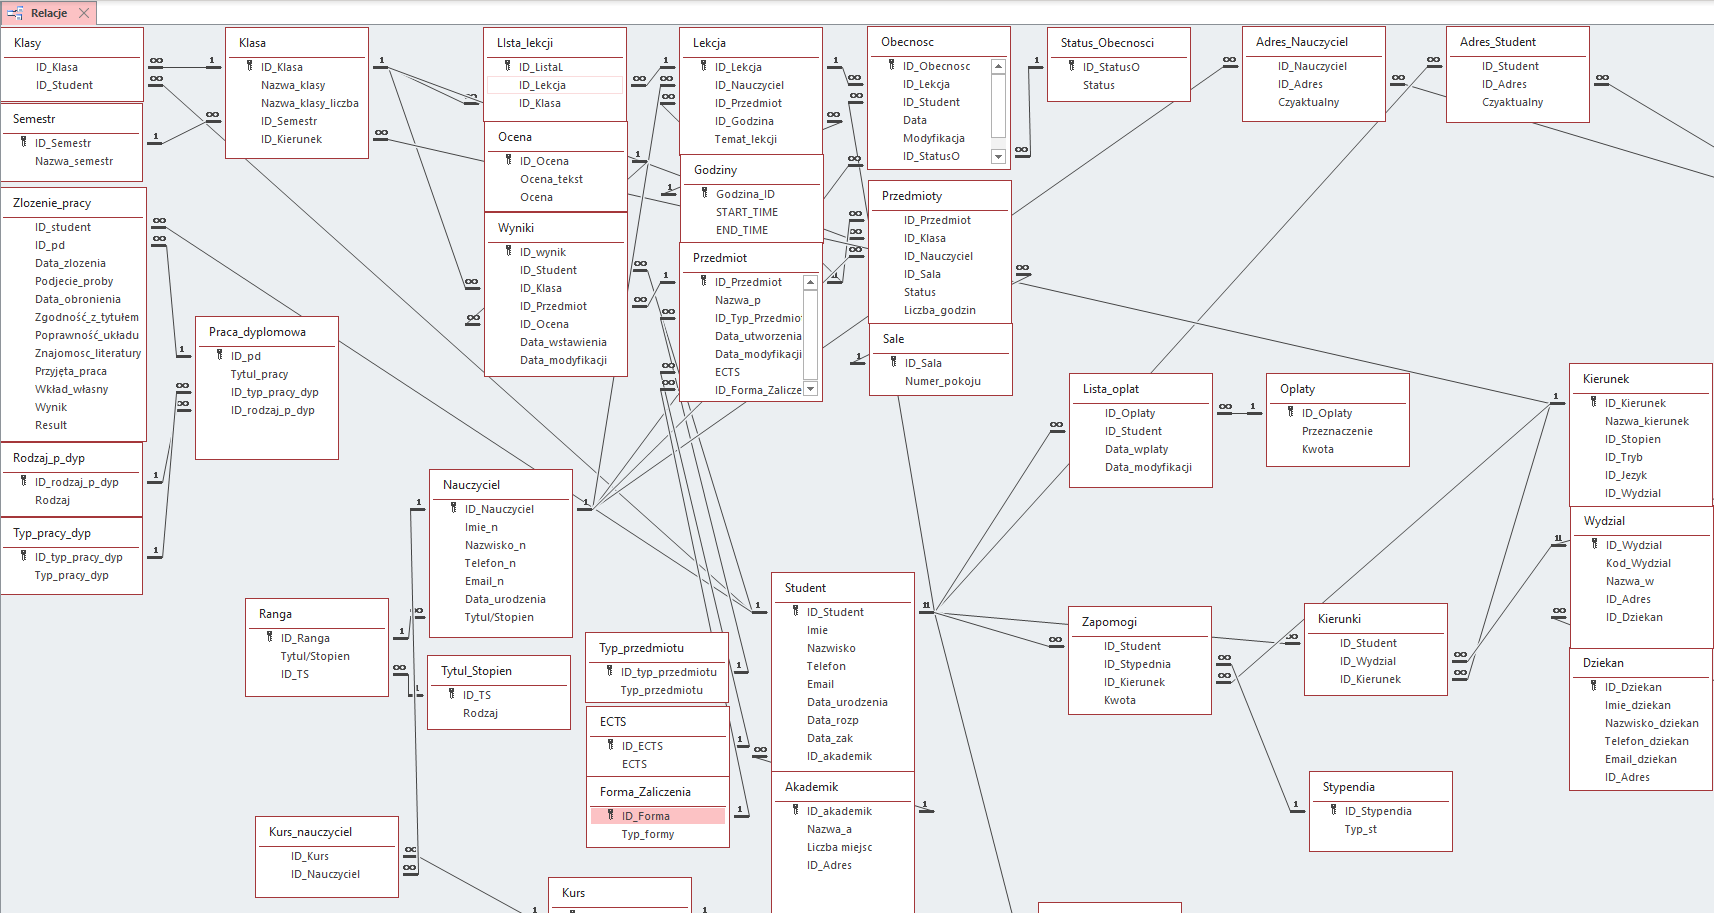
\includegraphics[scale=0.37]{Damian_Schroder_271395_ERD__cz1.png}\\
\newline
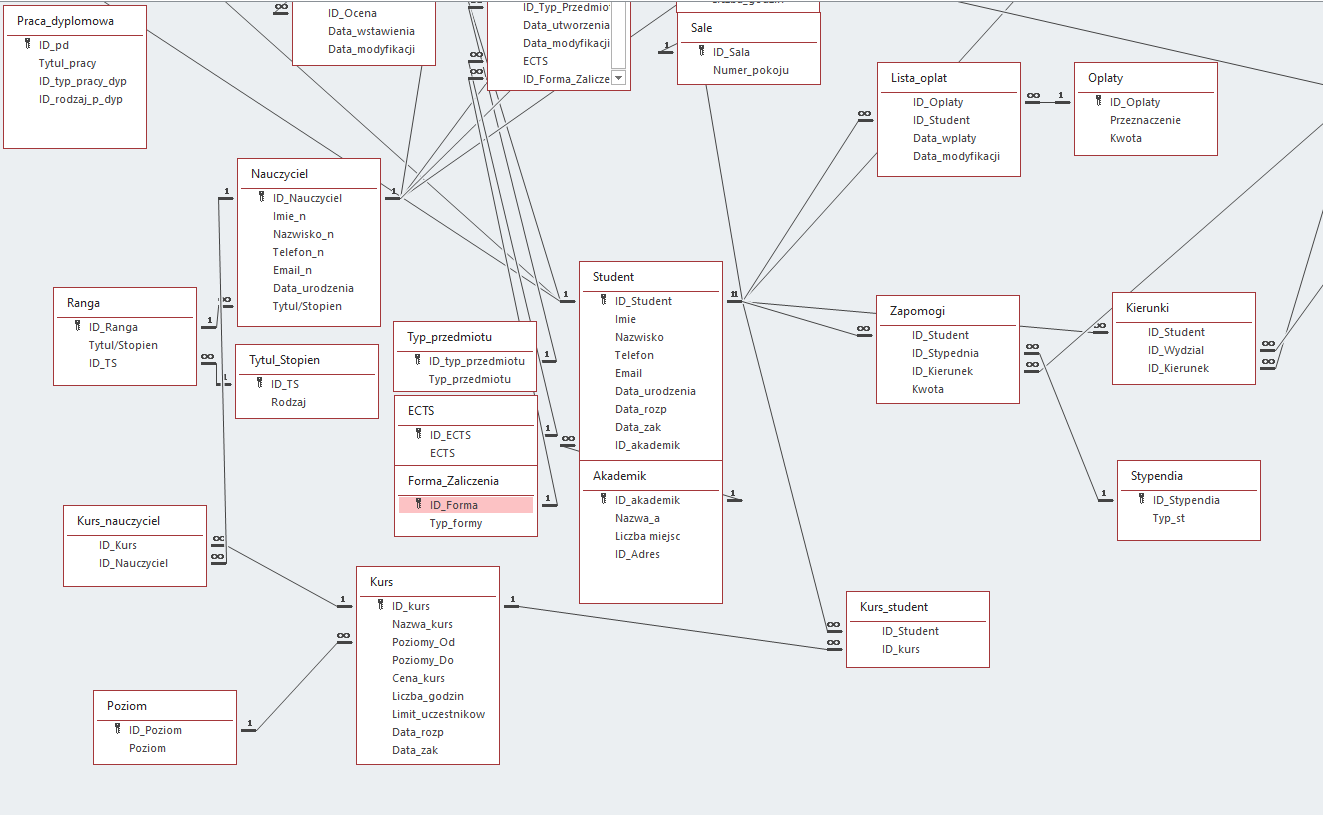
\includegraphics[scale=0.48]{Damian_Schroder_271395_ERD__cz2.png}\\
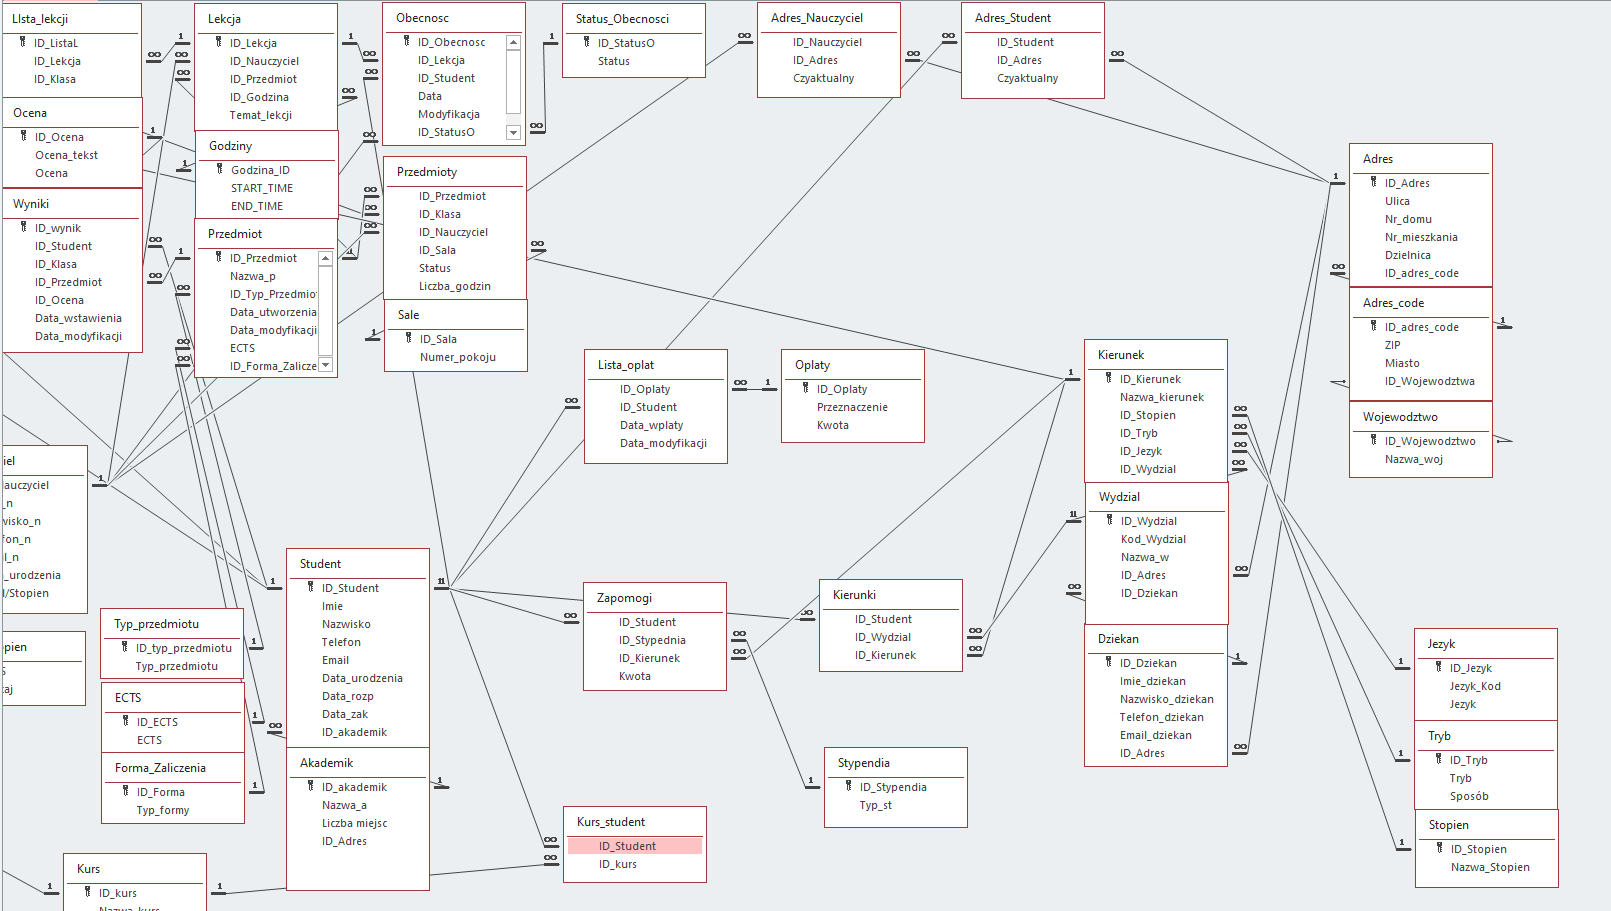
\includegraphics[scale=0.39]{Damian_Schroder_271395_ERD__cz3.png}\\


\section{Przykłady realizacji bazy danych}
\label{sec:ExamplesSection}
W pierwszej tabeli, dwa pola zostały zmodyfikowane:
\begin{itemize}
    \item Telefon - zawiera maskę wprowadzania, która zapobiega wprowadzaniu niechianych znaków,
    \item Email - generowany automatycznie na podstawie pierwszej litery imienia oraz nazwiska.
\end{itemize}
Pierwsze zapytanie zwraca studentów, klasy do których uczęszczają oraz przedmioty, jakie mają przypisane w danej klasie.
\newline

\noindent
Drugie natomiast zwraca średnią ocen z podziałem na klasy, do których są przypisani.

\subsection{Przykłady zawartości najważniejszych tabel}
\label{sec:ExampleTables}

Przykładową tabelę sql zamieszczamy przy pomocy polecenia \textbf{sqltable}:

\begin{sqltable}
+------------+--------------+------+-----+---------+-------+
| Field      | Type         | Null | Key | Default | Extra |
+------------+--------------+------+-----+---------+-------+
| ID_STUDENT | auto_inc	    | NO   | PRI | None    |       |
| IMIE 	    	| varchar(255) | NO   |     | None    |       |
| NAZWISKO   | varchar(255) | NO   |     | None    |       |
| TELEFON  	 | varchar(255) | NO   |     | None    |  yes  |
| EMAIL		     | varchar(255) | NO   |     | None    |  yes  |   
| DATA_URO	  | date   	     | NO   |     | None	   | 	     |  
| DATA_ROZP	 | date   	    	| NO   |     | None	   | 	     |
| DATA_ZAK	  | date   	    	| YES  |     | None	   | 	     |
| ID_AKADEMIK| int   	      | YES  | FOR | None	   | 	     |
+------------+--------------+------+-----+---------+-------+
\end{sqltable}

\begin{sqltable}
+------------+--------------+------+-----+---------+-------+
| Field      | Type         | Null | Key | Default | Extra |
+------------+--------------+------+-----+---------+-------+
| ID_OBECNOSC| auto_inc	    | NO   | PRI | None    |       |
| ID_LEKCJA	 | int		         | NO   | FOR | None    |       |
| ID_STUDENT | int		         | NO   | FOR | None    |       |
| DATA  	    | data		        | NO   |     | None    |   	   |
| MODYFIKACJA| data			        | NO   |     | None    |   	   |   
| ID_STATUSO | int   		      | NO   | FOR | None	   | 	     |  
| ID_NAUCZY	 | int   		      | NO   | FOR | None	   | 	     |
+------------+--------------+------+-----+---------+-------+
\end{sqltable}

\begin{sqltable}
+------------+--------------+------+-----+---------+-------+
| Field      | Type         | Null | Key | Default | Extra |
+------------+--------------+------+-----+---------+-------+
| ID_WYDZIAL | auto_inc	    | NO   | PRI | None    |       |
| KOD_WY	    | varchar(255) | NO   |     | None    |       |
| NAZWA		     | varchar(255) | NO   |     | None    |       |
| ID_ADRES 	 | int		         | NO   | FOR | None    |   	   |
| ID_DZIEKAN | int			         | NO   | FOR | None    |   	   |   
+------------+--------------+------+-----+---------+-------+
\end{sqltable}
\newpage
\begin{sqltable}
+------------+--------------+------+-----+---------+-------+
| Field      | Type         | Null | Key | Default | Extra |
+------------+--------------+------+-----+---------+-------+
| ID_PRZEDMI | auto_inc	    | NO   | PRI | None    |       |
| NAZWA		     | varchar(255) | NO   |     | None    |       |
| ID_TYP_PRZ | int          | NO   | FOR | None    |       |
| TELEFON  	 | varchar(255) | NO   |     | None    |       |
| DATA_UTW	  | date		        | NO   |     | None    |  	    |   
| DATA_MOD	  | date   		     | YES  |     | None	   | 	     |  
| ECTS		      | int   		      | NO   | FOR | None	   | 	     |
| ID_FORMA_Z | int   		      | NO   | FOR | None	   | 	     |
+------------+--------------+------+-----+---------+-------+
\end{sqltable}



\subsection{Przykłady kilku zapytań i ich wyników}
\label{sec:ExampleResults}

Przykłady umieszczamy przy użyciu specjalnych narzędzi do wstawiania kodu, a dokładniej pakietu \textbf{lstlisting}.

\begin{lstlisting}[language=SQL]
SELECT Student.Imie, Student.Nazwisko, Klasa.Nazwa_klasy, Klasa.ID_Semestr, Klasa.ID_Kierunek, Przedmiot.Nazwa_p, Przedmiot.ID_Typ_Przedmiotu
FROM Student INNER JOIN (Przedmiot INNER JOIN ((Klasa INNER JOIN Klasy ON Klasa.ID_Klasa = Klasy.ID_Klasa) INNER JOIN Przedmioty ON Klasa.ID_Klasa = Przedmioty.ID_Klasa) ON Przedmiot.ID_Przedmiot = Przedmioty.ID_Przedmiot) ON Student.ID_Student = Klasy.ID_Student
GROUP BY Student.ID_Student, Student.Imie, Student.Nazwisko, Klasa.ID_Klasa, Klasa.Nazwa_klasy, Klasa.ID_Semestr, Klasa.ID_Kierunek, Przedmiot.ID_Przedmiot, Przedmiot.Nazwa_p, Przedmiot.ID_Typ_Przedmiotu;

SELECT Student.Imie, Student.Nazwisko, Klasa.Nazwa_klasy, Klasa.ID_Semestr, Klasa.ID_Kierunek, Avg(Ocena.Ocena) AS ŚredniaOfOcena
FROM Student INNER JOIN (Przedmiot INNER JOIN (Ocena INNER JOIN (Klasa INNER JOIN Wyniki ON Klasa.ID_Klasa = Wyniki.ID_Klasa) ON Ocena.ID_Ocena = Wyniki.ID_Ocena) ON Przedmiot.ID_Przedmiot = Wyniki.ID_Przedmiot) ON Student.ID_Student = Wyniki.ID_Student
GROUP BY Student.ID_Student, Student.Imie, Student.Nazwisko, Klasa.ID_Klasa, Klasa.Nazwa_klasy, Klasa.ID_Semestr, Klasa.ID_Kierunek;


\end{lstlisting}

\bibliographystyle{amsplain}
\bibliography{references.bib}
\nocite{*}

\end{document}
